%%%%%%%%%%%%%%%%%%%%%%%%%%%%%%%%%%%%%%%%%%%%%%%%%%%%%%%%%%%%%%%%%%%%%%%
% Universidade Federal de Santa Catarina
% Biblioteca Universitária
%----------------------------------------------------------------------
% Exemplo de utilização da documentclass ufscThesis
%----------------------------------------------------------------------
% (c)2013 Roberto Simoni (roberto.emc@gmail.com)
%         Carlos R Rocha (cticarlo@gmail.com)
%         Rafael M Casali (rafaelmcasali@yahoo.com.br)
%%%%%%%%%%%%%%%%%%%%%%%%%%%%%%%%%%%%%%%%%%%%%%%%%%%%%%%%%%%%%%%%%%%%%%%
\documentclass{ufscThesis} % Definicao do documentclass ufscThesis

%----------------------------------------------------------------------
% Pacotes usados especificamente neste documento
\usepackage{graphicx} % Possibilita o uso de figuras e gráficos
\usepackage{color}    % Possibilita o uso de cores no documento
\usepackage{pdfpages} % Possibilita a inclusão da ficha catalográfica
\usepackage{listings}
\usepackage[utf8]{inputenc}
\usepackage{lipsum}
\usepackage{caption}
\usepackage{graphicx}
\usepackage{url}
\usepackage{bytefield} % draw memory table
% START maquina de estados
\usepackage{pgf}
\usepackage{tikz}
\usepackage{makecell} %breakcell
\usepackage[section]{placeins} %figures in sections

\usepackage{booktabs} % tabela abnt
\usepackage{rotating} % rotaciona
\hyphenation{op-tical}  % pras palavras não passarem da margem

\usetikzlibrary{arrows,automata}
% END maquina de estados
\usepackage[colorinlistoftodos,prependcaption,textsize=tiny]{todonotes}

\usepackage{listings}
\usepackage{color}

\definecolor{mygray}{rgb}{0.4,0.4,0.4}
\definecolor{mygreen}{rgb}{0,0.8,0.6}
\definecolor{myorange}{rgb}{1.0,0.4,0}

\lstset{
basicstyle=\tiny\sffamily\color{black},
commentstyle=\color{mygray},
frame=single,
numbers=left,
numbersep=5pt,
numberstyle=\tiny\color{mygray},
keywordstyle=\color{mygreen},
showspaces=false,
showstringspaces=false,
stringstyle=\color{myorange},
tabsize=1,
frame=bt
}

%----------------------------------------------------------------------
% Comandos criados pelo usuário
\newcommand{\meutodo}[1][]{\@latex@warning{TODO #1}}
\renewcommand{\lstlistingname}{Algoritmo}% Listing -> Algorithm
\renewcommand{\lstlistlistingname}{Lista de \lstlistingname s}% List of Listings -> List of Algorithms

%\newcommand{\afazer}[1]{{\color{red}{#1}}} % Para destacar uma parte a ser trabalhada
\newcommand{\itodo}[1]{{\todo[inline]{#1}}} % Para destacar uma parte a ser trabalhada
\newcommand{\figref}[1]{{Figura \ref{#1}}} % Para destacar uma parte a ser trabalhada
\newcommand{\tabref}[1]{{Tabela \ref{#1}}} % Para destacar uma parte a ser trabalhada
%\newcommand{\ABNTbibliographyname}{REFERÊNCIAS} % Necessário para abnTeX 0.8.2


%hack of doom to section*work


\usepackage{etoolbox}
% \patchcmd{<cmd>}{<search>}{<replace>}{<success>}{<failure>}
\patchcmd{\section}{\centering}{}{}{}

\let\flushleftsection\section% Copy updated non-centered definition of \section
\newcommand{\sectionscenter}{\let\section\centeredsection}% Switch to centered \section
\newcommand{\sectionsleft}{\let\section\flushleftsection}% Switch to flush left \section
\newcommand{\sectionsright}{\let\section\flushrightsection}% Switch to flush left \section



% facilitates the creation of memory maps. Start address at the bottom, end address at the top.
% syntax: \memsection{end address}{start address}{height in lines}{text in box}
\newcommand{\memsection}[4]{
\bytefieldsetup{bitheight=#3\baselineskip}    % define the height of the memsection
\bitbox[]{10}{
\texttt{#1}     % print end address
\\ \vspace{#3\baselineskip} \vspace{-2\baselineskip} \vspace{-#3pt} % do some spacing
\texttt{#2} % print start address
}
\bitbox{16}{#4} % print box with caption
}

%----------------------------------------------------------------------
% Identificadores do trabalho
% Usados para preencher os elementos pré-textuais
\instituicao[a]{Universidade Federal de Santa Catarina} % Opcional
\departamento[a]{Biblioteca Universitária}
\curso[o]{Programa de Graduação em Engenharia Eletrônica}
\documento[a]{Trabaho de Conclusão de Curso (TCC)} % [o] para dissertação [a] para tese
\titulo{KDev-Embedded}
\subtitulo{Plugin para desenvolvimento de sistemas embarcados} % Opcional
\autor{Patrick José Pereira}
\grau{Engenheiro}
\local{Florianópolis} % Opcional (Florianópolis é o padrão)
\data{27-31}{Março}{2017}
\orientador[Orientador\\Universidade Federal de Santa Catarina]{Prof. Dr. Danilo Silva}
%\coorientador[Coorientador\\Universidade ...]{Prof. Dr.}
\coordenador[Coordenador\\Universidade Federal Santa Catarina]{Prof. Dr. Djones Vinicius Lettnin}

\numerodemembrosnabanca{3} % Isso decide se haverá uma folha adicional
\orientadornabanca{sim} % Se faz parte da banca definir como sim
\coorientadornabanca{nao} % Se faz parte da banca definir como sim
\bancaMembroA{Prof. Dr. Danilo Silva\\Universidade Federal de Santa Catarina} %Nome do presidente da banca
\bancaMembroB{Prof. Dr. Djones Vinicius Lettnin\\Universidade Federal de Santa Catarina} 
\bancaMembroC{Prof. Dr. Leandro Buss Becker\\Universidade Federal de Santa Catarina}
%\bancaMembroD{Quarto membro\\Universidade ...}       % Nome do membro da Banca
%\bancaMembroE{Quinto membro\\Universidade ...}       % Nome do membro da Banca
%\bancaMembroF{Sexto membro\\Universidade ...}        % Nome do membro da Banca
%\bancaMembroG{Sétimo membro\\Universidade ...}       % Nome do membro da Banca

\dedicatoria{Este trabalho é dedicado aos meus colegas de classe e aos meus queridos pais.}

%\agradecimento{Agradeço aos colaboradores à execução do trabalho.}

\epigrafe{Vivaldi, Beethoven e Chopin não morreram. Simplesmente viraram musica.}{}

%%%%
\textoResumo{
O desenvolvimento de software para sistemas embarcados se encontra em constante evolução, adaptação e popularização das plataformas embarcadas resultante do aumento na sua capacidade de processamento, assim como na grande quantidade de recursos integrados, tais como diferentes protocolos de comunicação acesso a internet entre outros. Este avanço tem contribuído para o surgimento de diferentes aplicações tais como IoT (\textit{Internet of Things}), IoSM (\textit{Internet of Smart Things}) e IoIT (\textit{Internet of Important Things}). Os padrões estão sendo redefinidos, tanto quanto a tecnologia quanto a metodologia de desenvolvimento existentes, fazendo com que as indústrias aderissem a abordagens não ortodoxas em uma tentativa para acompanhar a evolução dos sistemas de hardware e realizarem tarefas de alto grau de complexidade (utilizando comunidades de desenvolvimento,  ferramentas de código aberto e etc.). O Objetivo deste trabalho é o desenvolvimento de uma ferramenta capaz de permitir ao desenvolvedor de sistemas embarcados a possibilidade de criar, editar e verificar seus projetos sem a necessidade do uso de outras ferramentas, além de relatar o desenvolvimento de tal ferramenta, elabora o contexto das atualizações que estão sendo realizadas dentro das grandes empresas.

\abreviatura{IoT}{\textit{Internet of Things}}
\abreviatura{IoST}{\textit{Internet of Smart Things}}
\abreviatura{IoIT}{\textit{Internet of Important Things}}
}

\palavrasChave{Sistemas embarcados. \textit{Open Source}. Desenvolvimento. IoT.}

%%%%
%% ATUALIZAR
\textAbstract{The development of software for embedded systems is constantly evolving, adapting and popularizing the embedded platforms, resulting from the increase in its processing capacity, as well as the large amount of integrated resources, such as different communication protocols, internet access and others. This advancement has contributed to the emergence of different applications, such as IoT (Internet of Things), IoSM (Internet of Smart Things) and IoIT (Internet of Important Things). Standards are being redefined as much as technology and the existing development methodology, causing industries to adhere to unorthodox approaches in an attempt to keep with the evolution of hardware systems and performing tasks of high complexity (using development communities , Open source tools, and so on). The objective of this work is the development of a tool that allows the embedded systems developer the possibility of creating, editing and verifying their projects without the use of other tools, besides reporting the development of such tool, elaborating the context of the updates that are being carried out within large companies.}
\keywords{Embedded Systems. \textit{Open Source}. Development. IoT.}

%----------------------------------------------------------------------
% Início do documento
\begin{document}
%--------------------------------------------------------
% Elementos pré-textuais
\capa
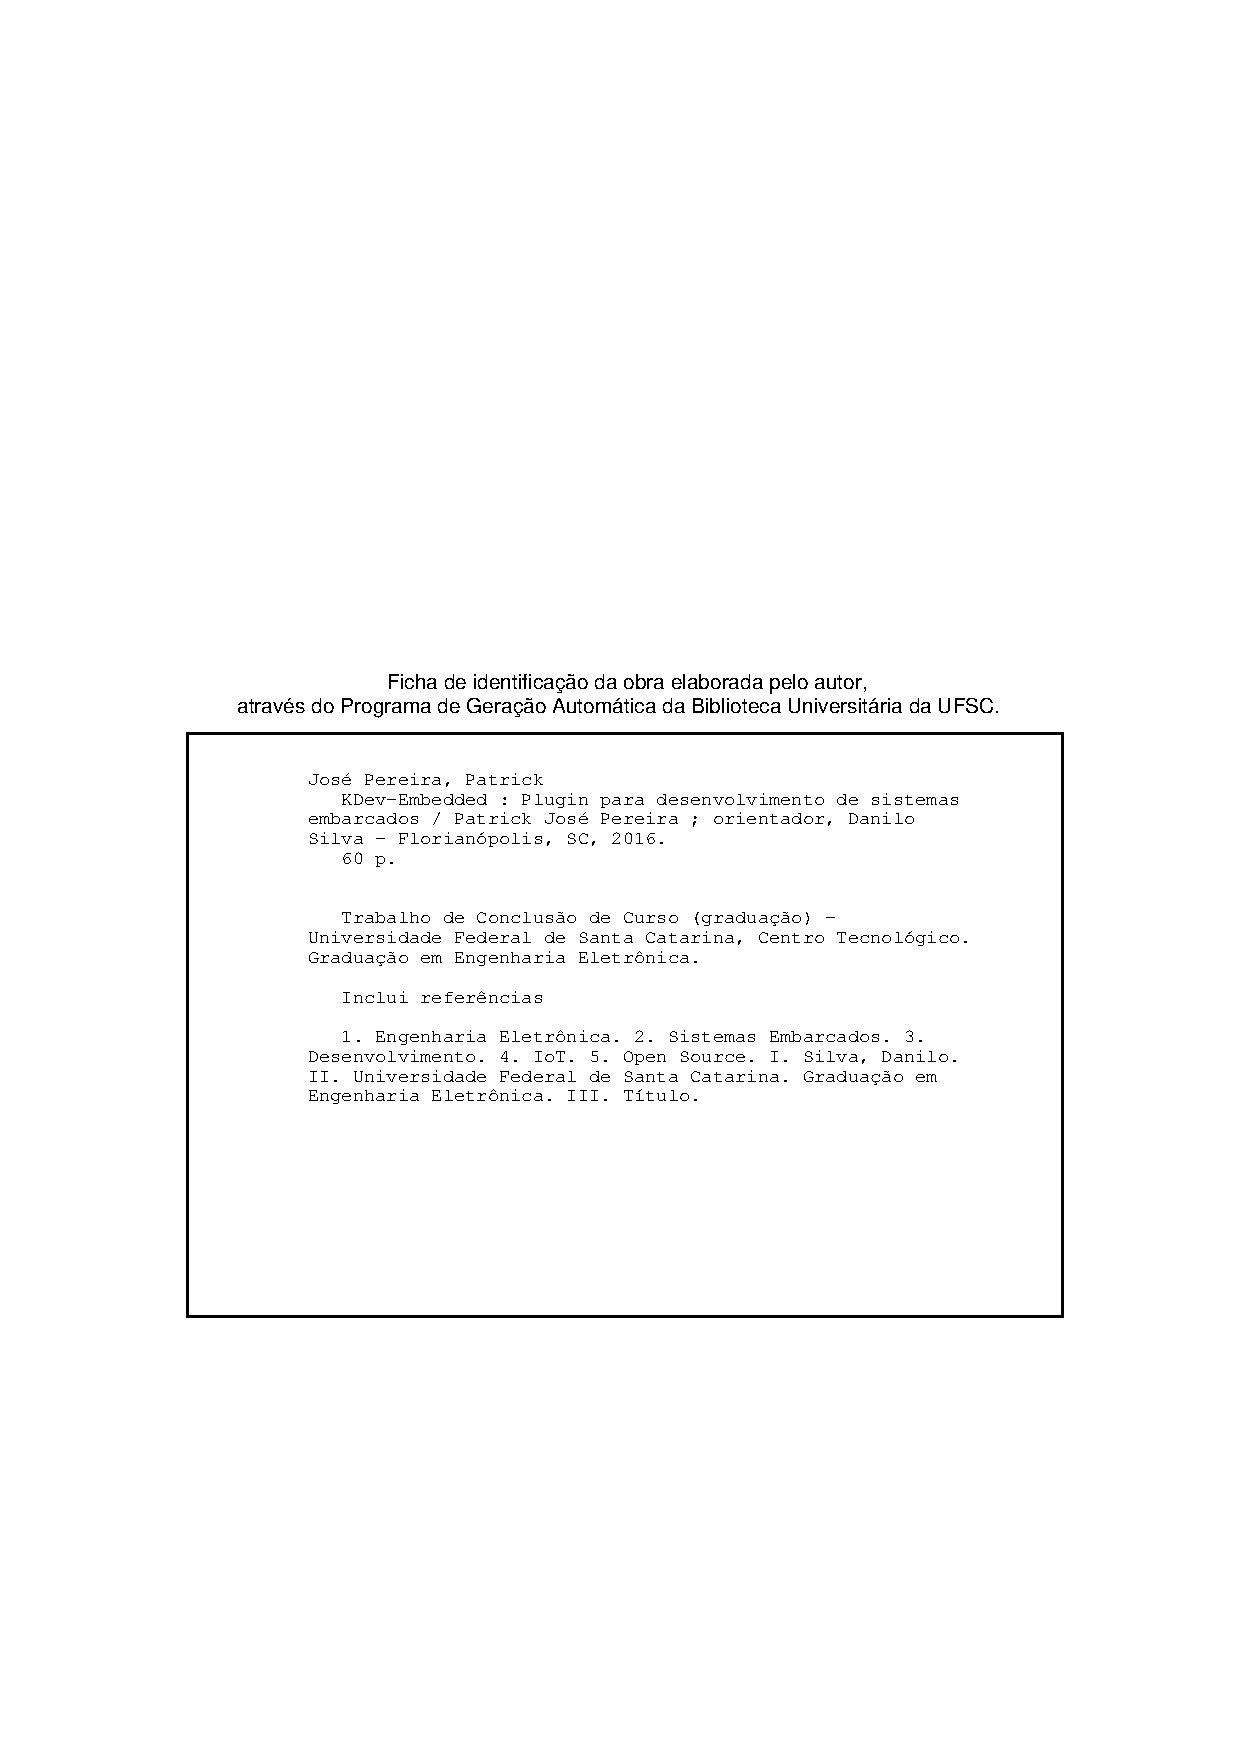
\includepdf{Ficha_Catalografica2.pdf}
%\folhaderosto[comficha] % Se nao quiser imprimir a ficha, é só não usar o parâmetro
\folhaaprovacao
\paginadedicatoria
\paginaagradecimento
\paginaepigrafe
\paginaresumo
\paginaabstract
%\pretextuais % Substitui todos os elementos pre-textuais acima
\listadefiguras % as listas dependem da necessidade do usuário
\listadetabelas
\listadeabreviaturas
\lstlistoflistings
%\listadesimbolos
\sumario
%--------------------------------------------------------
% Elementos textuais

\chapter{Introdução}
Nos últimos 40 anos existiram varias predições para o futuro da humanidade, conceitos como IoT(\textit{Internet Of Things})\cite{gates1995estrada} e ambiente ubíquo\cite{weiser1991computer} foram criados, propostas tecnológicas como a \textit{lei de Moore}\footnote{Citação famosa utilizada para Gordon Earle Moore, que tinha como proposta a duplicação do numero de transistores a cada 18 meses} eram ditas como garantidas pelos grandes fabricantes. Contudo muitos desafios acabaram prejudicando a execução destas predições, como, por exemplo, a barreira de potência\cite{Patterson:2008:COD:1502247} e a limitação de densidade energética\cite{paradiso2005energy}.
%http://www.singularity.com/charts/page70.html

Hoje, mesmo com desafios, o avanço tecnológico permitiu a miniaturização dos processadores com um custo de aquisição de grandezas menores das décadas anteriores\cite{nordhaus2007two}, possibilitando a pequenas empresas e até mesmo pessoas comuns o acesso a sistemas computacionais com alto processamento. Contudo, mesmo	 sendo possível, as ferramentas existentes para permitir o desenvolvimento desses processadores são geralmente pagas (\textit{IAR Embedded Workbench}\footnote{Não existe versão gratuita.}), limitadas (\textit{MDK Microcontroller Development Kit}\footnote{Versão gratuita com limite de código de 32 Kbytes.}) ou com poucos recursos (\textit{Platformio}\footnote{Sem depuração embutida.}).
%http://www2.keil.com/mdk5

A comunidade dos desenvolvedores de software para sistemas embarcados tende a utilizar inúmeras ferramentas para resolver os desafios de projeto, geralmente embutidas em uma IDE(\textit{Integrated Development Environment}), permitindo funções básicas, por exemplo, depuração, comunicação, gravação, entre outros. Algumas IDEs tendem a resolver mais de um problema ao mesmo tempo, resultando num sistema complexo, além disso, possuem a tendência de serem excessivamente assistencialistas (autocompletar e pop-ups sem requisição do usuário), abstraindo os sistemas que executam em segundo plano, resultando num uso maior do processador da maquina de trabalho, dificultando a personalização do fluxo de desenvolvimento e dos sistemas utilizados pelo desenvolvedor.

\iffalse
O intuito deste trabalho é a realização de um sistema para possibilitar aos desenvolvedores a programação de sistemas embarcados, sem a necessidade de utilizar sistemas assistencialistas que possam limitar a evolução do trabalho ou a utilização do produto final concebido.
\fi

O projeto tem como objetivo uma proposta de solução para os problemas descritos anteriormente, não providenciando alguma padronização ou mais uma alternativa entre as já existentes pelo mercado, mas uma IDE que tenha um suporte de alto nível para todos estes que já existem. Tendo como foco de usuário o desenvolvedor de sistemas embarcados, visando um ambiente configurável e mutável a suas necessidades.

Para a concepção, foi utilizado o KDevelop\footnote{IDE desenvolvida pela comunidade internacional de software livre KDE.} para base do sistema definido como proposta do GSoC (\textit{Google Summer Of Code})\footnote{Projeto de incentivo para estudantes no desenvolvimento de código livre organizado pela Google.}. Por ser uma IDE desenvolvida majoritariamente em C++ e permitir o carregamento em tempo de execução de algumas ferramentas (via a utilização de \textit{plugins}), já abrange alguns dos requerimentos do sistema que serão discutidos.

\section{Motivação}

Com o avanço tecnológico e a evolução do hardware heterogêneo (sistemas com GPU, CPU e outros periféricos), muitos dos sistemas disponíveis para desenvolvimento não seguem um padrão estabelecido no carregamento de código (gravador, protocolo, \textit{bootloader} e etc.), além disso, as empresas acabam criando alternativas aos padrões já
%https://community.nxp.com/thread/389162
 existentes no mercado ou opções limitadas, como, por exemplo, DebugWire\cite{debugwire}, hardware exclusivo de depuração LPC\cite{nxp}, suporte limitado de depuradores\cite{kiledebug} e etc, desta forma, dificultando ou restringindo o desenvolvimento.

\subsubsection{Ferramentas proprietárias}

Pela falta de um padrão definido, muitas empresas resolveram criar seus próprios, fundamentados em seus interesses ou na suas definições de utilização do que deveria ou não conter em suas soluções. Como consequência disso, são criados visões limitadas da realidade, resultante do modo de atuação interno vivida pela empresa, pela sua falta de conhecimento da realidade atual do mercado e suas utilizações.

Como consequência disso, a gama de padrões de protocolos de comunicação, \textit{bootloaders}, ICSPs, compiladores e outros materiais utilizados no desenvolvimento de sistemas embarcados, dificulta a realização do trabalho do desenvolvedor, principalmente se tais periféricos utilizados tem documentação e código fonte fechados, não permitindo seu conhecimento de funcionamento.

%\itodo{Adicionar footnote the bootloader}

\abreviatura{ICSP}{\textit{In Chip Serial Programmer}}

%\subsubsection{Padronização}

\section{Objetivo Geral}


%comment
\iffalse
O objetivo geral deve responder as seguintes perguntas:
1) O que a sua organização deseja realizar com o Projeto?
2) Qual problema em especial se quer solucionar?
3) Que mudanças se quer alcançar?
4) Que diferença o projeto quer fazer?

Deve ser escrito em tempo infinitivo (por exemplo: ampliar, capacitar, entre outros) e redigido com claridade. O objetivo precisa ser alcançável, não pode ser genérico, de forma que o projeto não consiga resolver (ex: terminar com a fome no mundo). Por outro lado deve ser ousado, capaz de sinalizar mudanças mais profundas que poderão ser alcançadas pelo projeto a médio e longo prazo.
\fi

\subsection{Metodologia}
\label{ss:objetivosespecificos}
Para realizar os objetivos, os seguintes passos são listados:
\begin{enumerate}
\item Estudo inicial d	as ferramentas utilizadas para desenvolvimento de sistemas embarcados.
\item Escolha das ferramentas inicialmente suportadas.
\item Estudo inicial sobre KDevelop.
\item Contato inicial com a comunidade do KDevelop%\footnote{adicionar nota de roda pé sobre o KDevelop, botar isso onde primeiramente acontece.} no irc \itodo{Adicionar abreviatura de irc} \footnote{Adicionar footnote sobre irc}.
\item Estudo para traçado inicial de estrutura e objetivo.
\item \textbf{Inicio do desenvolvimento}.
\item Carregamento do plugin.
\item Selecionar primeiro sistema embarcado para desenvolvimento.
\item Desenvolvimento do instalador de dependências.
\item Desenvolvimento de interface de programação.
\item Realização de testes utilizando o sistema selecionado.
\item Aprimoramento do sistema.
\item Selecionar outro sistema sistema embarcado para realizar o desenvolvimento.
\item Atualização do sistema de instalação.
\item Repetir passo 10 em diante.
\end{enumerate}

Todas as partes sitadas para a concepção do objetivo final, são de grande valia, tendo como maior importância o planejamento e a realização da primeira camada de software, este será o responsável pelo desenvolvimento do sistemas, e caso bem feito, todos os demais passos não deveram ter dificuldades para suas realizações e para futuras atualização do sistema proposto com novos sistemas embarcados.

\section{Estudo do fluxo de trabalho}

As tarefas descritas na subseção \ref{ss:objetivosespecificos} serão realizadas conforme a descrição feita das mesmas. A utilização dos resultados destes, serão integrados dentro do fluxo de trabalho de desenvolvimento incorporado na interface de desenvolvimento KDevelop, a mesma foi escolhida por ser uma das mais eficientes na sua velocidade de execução e de performance, possibilitando ao desenvolvedor que a utiliza o menor tempo de prototipagem comparado com as alternativas existentes.

A Filosofia da interface de projeto existente no KDevelop, permiti que boa parte das especificações de projeto fiquem nos sistemas de geração automatizada\footnote{Entre eles pode se destacar os mais utilizados são o \textit{Makefile}, \textit{CMakefile} e \textit{WAF}.}, permitindo ao programador o desenvolvimento de software sem a integração do projeto com a interface, utilizando arquivos intermediários de configuração\footnote{Arquivos que contem informações sobre compilador, estilo de código, execução e etc.}. Esta flexibilidade de integração de projetos no KDevelop acrescenta um grau de dificuldade na realização do plugin, pois as informações necessárias para o \textit{upload} do binário para o sistema embarcado necessita a localização do mesmo dentro do sistema onde está sendo desenvolvido, localização da porta de comunicação com o hardware e entre outras dificuldades. %\itodo{ADICIONAR MAIS INFORMAÇÕES DE FLUXO}

\section{Estrutura do Trabalho}

\begin{enumerate}
\item \textbf{Introdução} - Tema e contextualização do que será abordado no trabalho.
\item \textbf{Fundamentos teóricos} - Revisão dos assuntos abordados e necessários, fundamentais para realização do projeto.
\item \textbf{Estado da arte} - Comparação dos sistemas existentes que abordam o assunto e tentam aplicar uma proposta de solução.
\item \textbf{Projeto da Ferramenta} - Rascunhos iniciais de interface e arquitetura de software.
\item \textbf{Desenvolvimento} - Relato do trabalho realizado, contendo informações do projeto e seu andamento.
\item \textbf{Conclusão} - Exposição dos resultados.
\end{enumerate}
%\itodo{Expandir de forma mais detalhada}

\chapter{Fundamentos teóricos}
\lipsum[1-4]

\section{Sistema embarcado}
\lipsum[1-4]

\subsection{Microcontrolador, microprocessador e SoC}
\lipsum[1-4]

\subsection{Sistema de boot}
\lipsum[1-4]

\subsection{Gravação}
\lipsum[1-4]

\section{KDevelop}
\lipsum[1-4]

\subsection{Plugins}
\lipsum[1-4]

\subsection{Comunidade Open Source}
\lipsum[1-4]

\subsection{KDE}
\lipsum[1-4]

\section{Sistema de Controle de Versão}
\lipsum[1-4]


\chapter{Estado da Arte}
\lipsum[1-4]

\section{Ferramentas Existentes}
\lipsum[1-4]

\section{Dificuldades}
\lipsum[1-4]

\section{Evoluções}
\lipsum[1-4]


%http://www.linux-magazine.com/Online/Blogs/Paw-Prints-Writings-of-the-maddog/Brazil-Free-and-Open-Source-Culture-Is-Economics-Not-Politics
%https://books.google.com.br/books?id=pxAVCgAAQBAJ&pg=PA166&lpg=PA166&dq=Brazil:+Free+and+Open+Source+Culture+Is+Economics,+Not+Politics&source=bl&ots=k5M51pGklX&sig=tCPn4l7OnL7Xzne9cKYowUbYTvo&hl=pt-BR&sa=X&ved=0ahUKEwihkIec0-HPAhUGjpAKHdv6AcwQ6AEIOzAE#v=onepage&q=Brazil%3A%20Free%20and%20Open%20Source%20Culture%20Is%20Economics%2C%20Not%20Politics&f=false
%http://pear.accc.uic.edu/ojs/index.php/fm/article/view/904/813
%https://books.google.com.br/books?id=fEP2smsHVCwC&pg=PA14&lpg=PA14&dq=Brazil:+Free+and+Open+Source+Culture+Is+Economics,+Not+Politics&source=bl&ots=FsxRuW6joV&sig=l_PNwCwjTLl-XBATmeSIVO70Fcs&hl=pt-BR&sa=X&ved=0ahUKEwihkIec0-HPAhUGjpAKHdv6AcwQ6AEISzAG#v=onepage&q=Brazil%3A%20Free%20and%20Open%20Source%20Culture%20Is%20Economics%2C%20Not%20Politics&f=false
\chapter{Projeto da ferramenta}

KDE é conhecido por utilizar as ferramentas e bibliotecas disponibilizadas pela \textit{QT Project}\footnote{Empresa desenvolvedora  de software, famosa pelas suas bibliotecas e \textit{IDEs} de desenvolvimento} na realização do desenvolvimento dos seus projetos. O conhecimento inicial de como utilizar tais ferramentas é de grande valia para o projeto no desenvolvimento da proposta.


\section{Requisitos}

O usuário deve ser capaz de utilizar o plugin para realizar a programa-\\ção de sistemas embarcados, com a ajuda de um \textit{bootloader}, ou utilizando carregadores de código especializado do hardware. Além de ser possível programar, dependendo do caso, o desenvolvedor seria capaz de utilizar o plugin para a realização da depuração do projeto dentro do próprio sistema em desenvolvimento, caso o sistema utilizado por suportar tal comportamento.

A escolha do Arduino como plataforma alvo foi realizada pela sua fácil aquisição, baixo preço e alta popularidade dentre a comunidade civil como um dos microcontroladores mais populares, desta forma, é um bom primeiro passo para a realização da estrutura de software a ser desenvolvida para o plugin.

O sistema deve ter as seguintes funcionalidades para exercer um bom funcionamento para o usuário.
\begin{itemize}
\item O sistema deve permitir ao usuário:
	\subitem A criação de novos projetos e disponibilizar um modelo.
	\subitem Integração de projeto do usuário.
    \subitem Configuração das ferramentas utilizadas.
	\subitem Executar a compilação do projeto.
	\subitem Executar a instalação de ferramentas.
	\subitem Carregar o binário para o sistema embarcado.
\item Os projetos devem ser salvos assim como as configurações.
\item Executar o carregamento utilizando as ferramentas selecionadas.
\item Avisar sobre erros e problemas durante a ocorrência de alguma etapa para o usuário.	
\end{itemize}

Algumas propriedades e restrições do sistema são vitais para seu funcionamento.
\begin{itemize}
\item O sistema deve executar sem acarretar em uma falha durante a execução.
\item A instalação de ferramentas podem ser feitas sem a permissão de administrador.
\item O programa deve executar sem vazamento de memória \cite{Patterson:2008:COD:1502247}.
\item Evitar a manipulação do arquivo por terceiros durante a instalação das dependências.
\end{itemize}

\section{Plataformas suportadas}

Neste projeto, como versão inicial, será suportado as plataformas mais populares da Arduino, validando o suporte para placas com processadores AVR da plataforma, e os sistemas que utilizam \textit{OpenOCD}\footnote{Utilizando majoritariamente em placas com processadores ARM (Arduino DUE, STM32, entre outros).}, resultando num sistema que pode ser utilizado em todas as placas da Arduino\footnote{Com processadores ARM e AVR.}. Outros suportes para sistemas de carregamento podem vir a ser adicionados em futuras versões.


\section{Estrutura do software}

Foi desenvolvido um diagrama de classes (\figref{fig:uml}) que demonstra a proposta de software do plugin. A estrutura do Arduino \textit{toolkit} necessita de certas classes ou funções especiais para sua integração com a proposta do trabalho, além disso, certas classes foram feitas para as interfaces com foco nos usuários menos experientes. Outras camadas têm como proposta uma abstração para as placas de desenvolvimento, lidando com muitas variações de processador e configurações de hardware. 

Esta proposta inicial de UML seria realizada como prova de conceito da integração do KDevelop para sistemas embarcados, desta forma, necessitando de modificações para a criação de classes mais abstratas, permitindo uma melhor incorporação de outras ferramentas de desenvolvimento.o.

\begin{figure}[!htb]
  \centering
  \includegraphics[width=0.85\textwidth]{figuras/uml.png}
  \caption[UML proposto]{Representação do plugin proposto através do diagrama de classes UML.}
  \label{fig:uml}
\end{figure}

\abreviatura{UML}{Unified Modeling Language}


%Em futuras versões mais  ferramentas deverão ser adicionados,
%, serão os primeiros a serem suportados pelo plugin como prova de conceito por apresentarem uma grande quantidade de usuários.
%Como objetivo final do projeto, o usuário deve ser capaz de utilizar o


\chapter{Desenvolvimento}
\lipsum[1-4]

\section{EXPOSIÇÃO DO TEMA OU MATÉRIA}
\lipsum[1-4]

\subsection{Ferramentas Utilizadas}
\lipsum[1-4]

\subsection{Protótipo de funcionamento}
\lipsum[1-4]

\subsection{Integração com KDevelop}
\lipsum[1-4]

\section{Integração com fluxo de trabalho}
\lipsum[1-4]


\chapter{Conclusão}
\lipsum[1-4]

\section{Contribuições}
\lipsum[1-4]

\section{Futuros}
\lipsum[1-4]

\section{Trabalhos de Pesquisa}
\lipsum[1-4]


\bibliographystyle{unsrt}
\bibliography{bibliografia}

%\iffalse
%--------------------------------------------------------
% Elementos pós-textuais
%\apendice
%\chapter{Exemplificando um Apêndice}
%Texto do Apêndice aqui.

%\anexo
%\chapter{Código do plugin}

%\lstinputlisting[language=C++,caption={arduinowindow.h},label=DescriptiveLabel]{kdev-embedded/arduinowindow.h}
%\lstinputlisting[language=C++,caption={arduinowindow.cpp},label=DescriptiveLabel]{kdev-embedded/arduinowindow.cpp}
%\lstinputlisting[language=C++,caption={toolkit.h},label=DescriptiveLabel]{kdev-embedded/toolkit.h}
%\lstinputlisting[language=C++,caption={toolkit.cpp},label=DescriptiveLabel]{kdev-embedded/toolkit.cpp}
%\lstinputlisting[language=C++,caption={firsttimewizard.h.in},label=DescriptiveLabel]{kdev-embedded/firsttimewizard.h.in}
%\lstinputlisting[language=C++,caption={firsttimewizard.cpp},label=DescriptiveLabel]{kdev-embedded/firsttimewizard.cpp}
%\lstinputlisting[language=C++,caption={embedded.h},label=DescriptiveLabel]{kdev-embedded/embedded.h}
%\lstinputlisting[language=C++,caption={embedded.cpp},label=DescriptiveLabel]{kdev-embedded/embedded.cpp}
%\lstinputlisting[language=C++,caption={board.h},label=DescriptiveLabel]{kdev-embedded/board.h}
%\lstinputlisting[language=C++,caption={board.cpp},label=DescriptiveLabel]{kdev-embedded/board.cpp}
%\if
\end{document}
